\SetVertexNormal[Shape      = circle,
                 FillColor  = orange,
                 LineWidth  = 1.5pt]
\SetUpEdge[lw         = 1pt,
           color      = black,
           labelcolor = white,
           labeltext  = black,
           labelstyle = {sloped,draw,text=blue}]
\begin{center}
\begin{tikzpicture}
   \Vertex[x=-1,y=0]{S}
   \Vertex[x=11 ,y=0]{T}
   \Vertex[x=5,y=0]{Z}
   \Vertex[x=1 ,y=1]{A}
   \Vertex[x=3 ,y=2]{B}
   \Vertex[x=5 ,y=2]{C}
   \Vertex[x=7 ,y=2]{D}
   \Vertex[x=9 ,y=1]{E}
   \Edge[label = $12$,color=gray](S)(Z)
   \Edge[label = $10$,color=gray](Z)(T)   
   \Edge[label = $1$](S)(A)
   \Edge[label = $2$](A)(B)
   \Edge[label = $3$](B)(C)
   \Edge[label = $4$](C)(D)
   \Edge[label = $5$](D)(E)
   \Edge[label = $6$](E)(T)
\end{tikzpicture}\\
{\small El camino superior tiene longitud 21, mientras que el inferior 22.}
\end{center}